\documentclass[12pt]{article}
\usepackage[papersize={8.5in,11in}]{geometry}
\usepackage[pdftex]{graphicx}
\DeclareGraphicsExtensions{.pdf,.png,.jpg}
%
\usepackage{amsmath}
\usepackage{amsthm}
\usepackage{amssymb}
\usepackage{textcomp}
\usepackage[all]{xy}
\usepackage{fancyhdr}
\usepackage{hyperref}
\usepackage{verbatim}
\usepackage{algorithm}
\usepackage{algorithmic}
\usepackage{color}
\usepackage[usenames,dvipsnames,svgnames,table]{xcolor}
\usepackage{rotating}
\usepackage{wrapfig}
\usepackage{tikz}
\usetikzlibrary{shapes.geometric, arrows}
\usepackage{framed}
\usepackage[scaled=0.75]{FiraMono}
%\usepackage{newtxtt}

\usepackage{listings}
\lstset{language=python,frame=ltrb,framesep=5pt,basicstyle=\ttfamily,
 keywordstyle=\ttfamily\color{DarkRed}\bfseries,
%morecomment=[n][\textbf]{In\ [}{]\:},
%morecomment=[n][\textbf]{Out\ [}{]\:},
morecomment=[s][\color{blue}]{In\ [}{]\:},
morecomment=[s][\color{red}]{Out[}{]\:},
identifierstyle=\ttfamily\color{DarkBlue},
commentstyle=\color{OliveGreen},
stringstyle=\ttfamily\color{Orange},
showstringspaces=false,tabsize = 3}

\lstdefinelanguage{shell} {
commentstyle = \color{black},
keywordstyle = \color{black},
stringstyle = \color{black},
identifierstyle = \color{black},
morecomment=[s][\color{blue}]{In\ [}{]\:},
morecomment=[s][\color{red}]{Out[}{]\:},
 }


%
% this gives a little box for the end of a proof:
%
\def\endthrmbox{$\sqsubset \!\!\!\! \sqsupset$}

\newcommand{\dis}{\displaystyle}
 \def      \RR             {{\mathbb R}}
        \def      \NN             {{\Bbb N}}
        \def      \QQ             {{\Bbb Q}}
        \def      \CC             {{\Bbb C}}
        \def      \ZZ             {{\Bbb Z}}


        \def       \a              {{\alpha}}
        \def       \b              {{\beta}}
        \def       \d              {{\delta}}
        \def       \D              {{\Delta}}
        \def         \e              {{\varepsilon}}
        \def         \g              {{\gamma}}
        \def         \G              {{\Gamma}}
        \def       \l              {{\lambda}}
        \def       \L              {{\Lambda}}
        \def        \m               {{\mu}}
        \def         \n              {{\nabla}}
        \def       \var          {{\varphi}}
        \def         \s              {{\sigma}}
        \def       \Sig          {{\Sigma}}
        \def       \Om          {{\Omega}}

        \def       \t              {{\tau}}
        \def         \th             {{\theta}}
        \def       \O              {{\Omega}}
        \def       \o              {{\omega}}
        \def         \z              {{\zeta}}
       \def        \P             {{\Phi}}
       \def        \p             {{\phi}}
        %Other macros

        \def       \iy              {{\infty}}
        \def         \pa             {{\partial}}
        \def         \div           {{\rm div}}
         \def       \na            {{\nabla}}


%\renewcommand\baselinestretch{1.3}
%% The following block is for narrow margins:
\setlength{\topmargin}{-0.9in}
\setlength{\textheight}{9.50in}
\setlength{\oddsidemargin}{-0.375in}
\setlength{\evensidemargin}{-0.375in}
\setlength{\textwidth}{7.25in}
\setlength{\parindent}{0pt}
\setlength{\parskip}{2pt}
%% end page descript.




\usepackage[compact,explicit]{titlesec}
\titleformat{\section}[runin]{\large\bfseries}{}{0pt}{\titlerule[1.5pt]\newline\vspace*{-4pt}\quad
\newline}%[\vspace{0.01ex}{\titlerule[1.5pt]}]

\usepackage[final]{pdfpages}

\title{Homework \#2}
\author{Kyle MacMillan, \\Remington Bullis}


\begin{document}
\maketitle

Having now had a half-semester to digest and process information about nature-inspired computing approaches like simulated annealing and various implementations of evolutionary algorithms, Homework \#2 challenged us to tackle a nontrivial task: image reproduction. Our official bidding was to use an evolutionary algorithm (with our own quirks)  to evolve the closest approximation of a given image. Our implementation focused on a very robust generation-to-generation reproduction system using both crossover and point mutations. This approach yielded remarkable results. 
\\ \\
\textbf{Note: }The repository for this paper can be found \href{https://github.com/macattackftw/ncGA}{here}. 
The \verb|README.md| contains a gif of our solution in action and a full suite of test results can be seen in the \verb|results| folder. A selection of these results can also be seen in Appendix A. 

\section{} %%  This will generate a numbered problem header.

\subsection{Initial Approach and Encoding}
Before programming could begin we needed to know \textbf{1)} the language with which we would write our project, and \textbf{2)} the exact algorithm we were implementing. Python was the obvious choice for quickly iterating and testing. Algorithm development started at the discussion of how exactly we were going to generate images. After some back and forth we decided to build our image reconstructions purely in grayscale, and with layered circles. One "epoch" would be completed to generate an optimal circle. Each epoch would consist of its own population which was to be evolved over a set number of generations, with the most fit individual pulled and added to the reconstruction. While computationally intensive this one-at-a-time approach was expected to be robust and consistently convergent. 
\\
Encoding the properties of a circle into a genome was quite simple. We used \verb|numpy| to define a datatype that held the following information:
\begin{itemize}
\item The circle's center coordinates, $(x, y)$
\item The circle's radius, $r$
\item the circle's intensity, or alpha value, $i$
\end{itemize}

The actual definition of our genome can be seen below:
\begin{lstlisting}
self.center = np.dtype([('x', np.float32), ('y', np.float32)])
self.genome = np.dtype([('center',self.center), ('radius', np.float32), ('intensity', np.float32) ])
\end{lstlisting}


\subsection{Measuring Individual Fitness}
Given a circle to be placed on the stack of circles, how do we determine how "fit" this individual is relative to any other circle? This question plagued us for days. Unlike a simple mathematical function one can't just plug a circle into an image and get a numeric out indicating progress. The circle's fitness depends on not only the information confined to its bounds, but also how the circle fits into the larger context of the image. Our initial approaches to generating a fitness function proved fruitless; one simply filled the image as quickly as possible with white, and another would produce results only slightly better than random circle placement. 

We eventually determined that, given a circle, we should:
\begin{enumerate}
\item Determine the number of pixels occupied by the circle, $n$
\item Generate the circle in a mask
\item Add this mask to the current circle stack, constructing  a prospective next-circle stack
\item Determine the total difference between this prospective stack and the actual image to be reconstructed. This is $e$
\item Calculate an offset to linearly shift fitness against circle size
\item Return a final fitness $e - n*scale$, where scale is determined by the number of total pixels in the image 
\end{enumerate}

Our function definition is as follows:
\begin{lstlisting}
def Fitness(self, individual):
  cx, cy, r = individual['center']['x'], individual['center']['y'], individual['radius']
  Y, X = np.ogrid[-cy:self.height - cy, -cx:self.width - cx]
  mask = X**2 + Y**2 <= r**2                   # Calculate mask
  # Where the magic begins
  pixel_count = np.sum(mask, dtype=np.float32)
  circle = mask * individual['intensity']
  art = self.art + circle 						     # Gen prospective stack

  return np.sum(np.abs(self.image - art)) - pixel_count * self.pixel_modifier
\end{lstlisting}

This fitness function proved to be the key to convergence. Once we had it in place, the stars aligned!

\subsection{Evolving a New Circle}

\subsubsection{Mutation and Crossover}

\subsubsection{Selection}

\subsection{Results}

\subsection{Conclusions}

\begin{figure}[H]
\centering
\noindent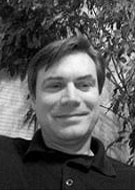
\includegraphics[width=0.65\textwidth]{../images/jmcgough}
\caption{The Persistence of Memory}
\label{fig:jmcgough}
\end{figure}

\begin{figure}[H]
\centering
\noindent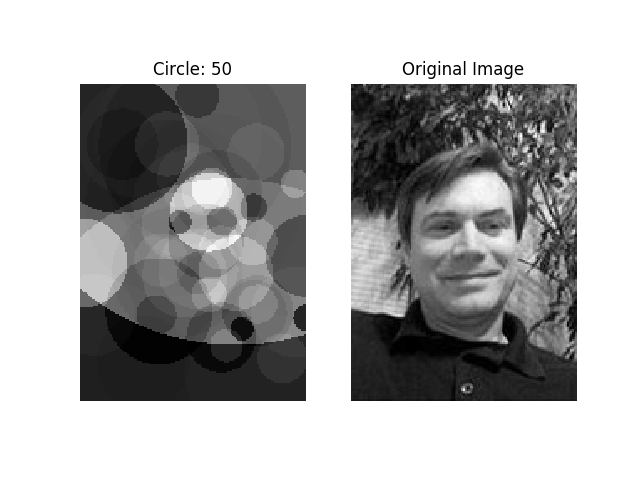
\includegraphics[width=0.65\textwidth]{../results/jmcgough/jmcgough_0050.png}
\caption{\textit{The Persistence of Memory} with 50 circles}
\label{fig:jmcgough_0050}
\end{figure}

\begin{figure}[H]
\centering
\noindent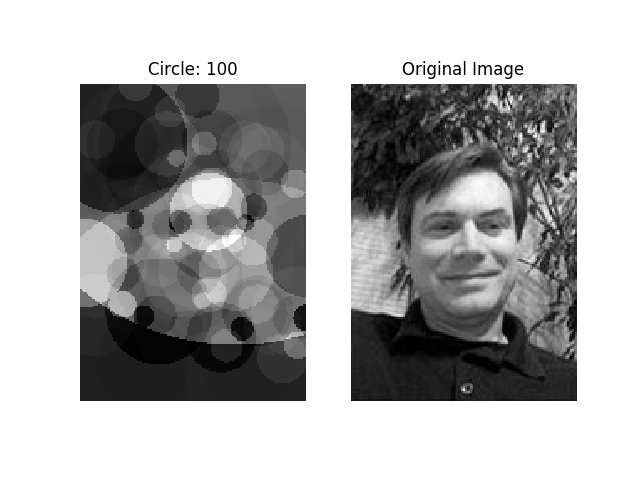
\includegraphics[width=0.65\textwidth]{../results/jmcgough/jmcgough_0100.png}
\caption{\textit{The Persistence of Memory} with 100 circles}
\label{fig:jmcgough_0100}
\end{figure}

\begin{figure}[H]
\centering
\noindent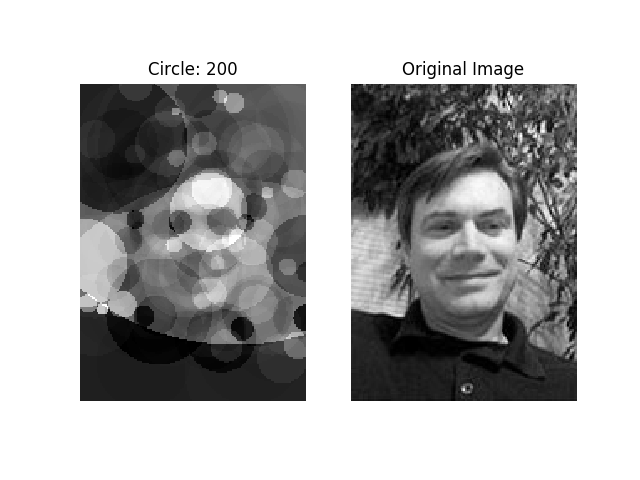
\includegraphics[width=0.65\textwidth]{../results/jmcgough/jmcgough_0200.png}
\caption{\textit{The Persistence of Memory} with 200 circles}
\label{fig:jmcgough_0200}
\end{figure}



\newpage
\subsection{Code}
\subsubsection{Best Circle}
\begin{lstlisting}
import numpy
\end{lstlisting}


\end{document}
